\documentclass[twocolumn]{iopjournal}

\usepackage{amsmath,amssymb,amsfonts}

\fancyhfoffset[L]{0mm}
\setlength{\marginparwidth}{0pt}
\setlength{\marginparsep}{0pt}

% ==========================================
% ZENODO PREPRINT HEADERS (ACTIVE)
% ==========================================
\renewcommand{\articletype}[1]{%
  {\vspace*{-8mm}\noindent \Large \sf Preprint}\par
  \vspace*{6mm}\noindent{\scriptsize \sf{\bfseries \MakeUppercase{#1}}}}

\fancyhead[L]{}
\fancyhead[R]{}

% ==========================================
% CQG SUBMISSION HEADERS (COMMENTED OUT)
% ==========================================
% \fancyhead[L]{{\small \sf IOP Publishing}\hspace{5mm} {\it Class. Quantum Grav.}}
% \fancyhead[R]{S Nelson}

\begin{document}

\articletype{Letter}

\title{Gravity Field Dynamics and Bimetric Gravity: Dual Tetrahedral Field Chambers as the Key to the General Parameters}

\author{Stephen Nelson}

\affil{Field Dynamics Research}

\begin{abstract}
Bimetric gravity provides a theoretically robust, ghost-free framework for interacting spin-2 fields, yet its interaction potential has remained phenomenologically underdetermined for over a decade: the five coefficients $\beta_n$ have been treated as continuous free parameters to be fitted to cosmological data. We show that Gravity Field Dynamics (GFD), the derivation of gravitational coupling laws from the discrete combinatorial geometry of the local tetrad frame, resolves this underdetermination. The GFD coupling polynomial $f(k,s) = 1 + ks + k^2$, evaluated at $k = 4$ tetrahedral faces, encodes the full interaction structure: its static skeleton at the symmetric point ($s = 0$) yields the locked integer coefficients $\{\beta_n\} = \{1, 0, 16, 0, 1\}$, while its dynamic body under the conformal map $s(x) = (x-1)/(x+1)$ produces the continuous topological capacity $f(x) = (21x + 13)/(x + 1)$. Normalizing this capacity recovers the constitutive law $\mu(x) = x/(x+1)$ and determines the scalar-tensor action without fitted parameters. Within GFD, the UV bimetric potential and the IR scalar-tensor action are projections of a single geometric object: the topological capacity of the dual tetrahedral field chamber. The locked potential lies within the ghost-free Hassan--Rosen class by construction.
\end{abstract}

% ----------------------------------------------------------------------

\section*{Introduction: From Framework to Theory}

\subsection*{The Tetrad Foundation}

General relativity is most commonly written in terms of the metric tensor $g_{\mu\nu}$, a symmetric matrix that encodes distances and angles in curved spacetime. However, there is a deeper formulation: the \emph{tetrad} (or \emph{vierbein}) formulation, in which the fundamental object is not the metric itself but a set of four vector fields $e^a{}_\mu$ that serve as a local orthonormal frame at each point. The metric is recovered as a derived quantity: $g_{\mu\nu} = \eta_{ab}\, e^a{}_\mu\, e^b{}_\nu$. The tetrad is, in a precise algebraic sense, the ``square root'' of the metric.

This is not an alternative theory of gravity. It is general relativity rewritten in a form that is strictly more fundamental: one cannot couple fermions (electrons, quarks, neutrinos, the matter content of the universe) to gravity without the local Lorentz frame that only the tetrad provides. The tetrad formulation has been standard since the work of Cartan, Einstein (1928), and Weyl (1929), and is essential to modern approaches including Ashtekar variables, loop quantum gravity, and supergravity. Despite its centrality, the tetrad formalism is almost always presented in index notation ($e^a{}_\mu$ carrying a Lorentz index and a spacetime index) without visualizing the geometric object these indices describe. In what follows, we write the tetrad explicitly as a spatial structure and show that making this geometry visible resolves a long-standing open problem in bimetric gravity.

\subsection*{Two Tetrads, Five Free Parameters}

Since the seminal work of Hassan and Rosen (2012), bimetric gravity has provided a consistent, ghost-free framework for coupling two dynamical spin-2 fields. In the tetrad formulation, the theory contains two independent tetrad fields, $e^a{}_\mu$ and $\tilde{e}^a{}_\mu$, each generating its own metric and propagating via its own Einstein--Hilbert kinetic term.

The interaction between the two tetrads must be a generally covariant, derivative-free scalar density. Covariance and the antisymmetry of the exterior product force this interaction to decompose into exactly five algebraic invariants, the elementary symmetric polynomials $e_n(S)$ of the frame transition matrix $S = e^{-1}\tilde{e}$, weighted by five coefficients $\beta_n$:
\begin{equation}
V = \sum_{n=0}^{4} \beta_n\, e_n(S).
\end{equation}

Hassan and Rosen proved that this potential is free of the Boulware--Deser ghost (a pathological extra degree of freedom that would render the vacuum unstable) for \emph{any} choice of the five $\beta_n$. The \emph{form} of the interaction is uniquely fixed by consistency. The \emph{values} of the five coefficients are not.

\subsection*{The Geometric Hardware: TetA, TetB, and the Interaction Vertex}

The tetrad literature consistently identifies the smallest volume-enclosing unit of local spatial geometry as the tetrahedron. In the bimetric context, the coupling involves three geometric elements:

\begin{itemize}
\item \textbf{TetA ($e$):} The primary local tetrad frame, a tetrahedron with $k = 4$ faces.
\item \textbf{TetB ($\tilde{e}$):} The inverted dual tetrad, required independently by chirality, fermionic stability, and ghost freedom.
\item \textbf{The interaction vertex:} The shared field origin where the two tetrahedral units couple face-to-face with opposite spatial orientations.
\end{itemize}

These three elements are not new theoretical postulates. They are implicit in every tetrad-based formulation of bimetric gravity. What has not previously been extracted is the consequence of their combinatorial geometry for the five $\beta_n$.

\subsection*{What a Tetrad Looks Like in Coordinate Space}

A tetrad is a set of four vector fields. In the local orthonormal frame, the spatial components of a regular tetrad point along four directions: the four face normals of a tetrahedron. These directions can be written as four linear projections of the local coordinates:
\begin{align}
v_1 &= x + y + z, \nonumber \\
v_2 &= x - y - z, \nonumber \\
v_3 &= -x + y - z, \nonumber \\
v_4 &= -x - y + z.
\end{align}
The primary field chamber (TetA) is the region where all four projections are bounded:
\begin{equation}
\text{TetA}: \quad \max(v_1,\, v_2,\, v_3,\, v_4) \leq 1.
\end{equation}
The inverted dual (TetB) satisfies the opposite inequality:
\begin{equation}
\text{TetB}: \quad \max(-v_1,\, -v_2,\, -v_3,\, -v_4) \leq 1.
\end{equation}
Their intersection is the central octahedral region, the Field Origin. Their union is a stellated octahedron.

\begin{figure}[t]
\centering
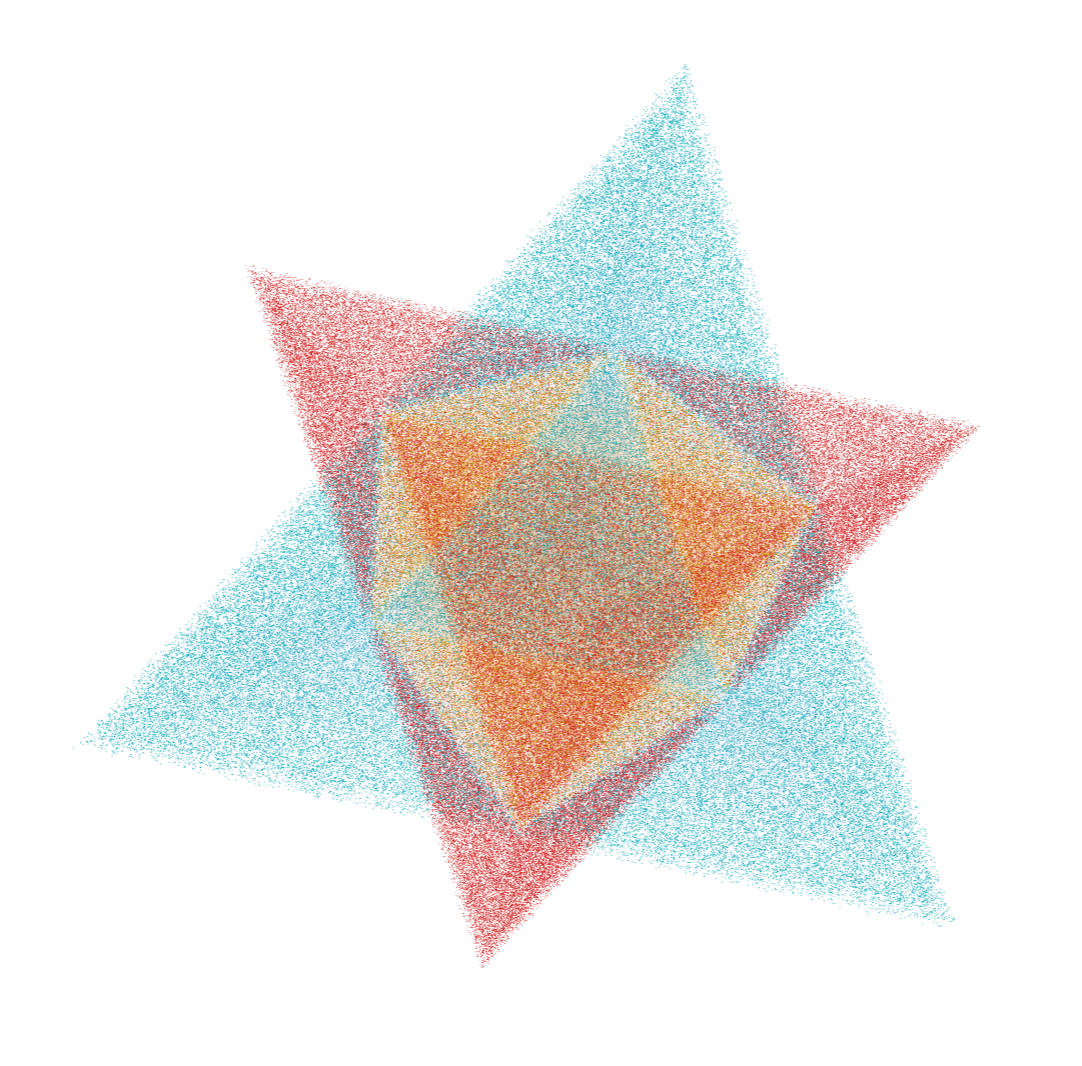
\includegraphics[width=\columnwidth]{fig1_dual_tetrahedral_field_chamber}
\caption{The dual tetrahedral field chamber. Four million points are sampled uniformly in local frame coordinates and tested against the half-space inequalities $L_i(\mathbf{p})$ defined in the text. Points that satisfy the TetA bounds are shown in cyan; those satisfying TetB in red; and those inside both (the shared octahedral Field Origin) in gold. No mesh or curve fitting is used. Each face of TetA is subdivided into three exposed corners and one inverted core where the opposing vertex penetrates, giving $4 \times 4 = 16$ geometric channels. These channels determine the bimetric interaction potential. An interactive reconstruction is provided as supplementary material.}
\label{fig1}
\end{figure}

Figure~\ref{fig1} shows the result of evaluating these half-space inequalities at four million randomly sampled points in local frame coordinates. No mesh is constructed; the geometry emerges from the boundaries alone. On each face of TetA, the penetration by TetB's opposing vertex subdivides the surface into four sub-regions: three spatial corners and one central inverted core. This $3 + 1$ subdivision, repeated across all four faces, produces exactly $4 \times 4 = 16$ independent boundary channels. The channel count is visible in the figure before it is proven in the derivation.

These four directional projections are the spatial content of the tetrad one-forms, the same objects from which both the bimetric action and the scalar-tensor action are built. Gravity Field Dynamics (GFD; foundational derivation provided in the supplementary material) contributes the recognition that writing them down as explicit half-space inequalities makes the interaction geometry computable and its channel structure visible.

\subsection*{The Open Problem}

Despite the geometric structure visible in Figure~\ref{fig1}, the five coefficients $\beta_n$ have been treated for over a decade as phenomenological tuning parameters, continuous real numbers to be constrained by fitting to supernova surveys, baryon acoustic oscillations, CMB data, and gravitational wave observations. Different research groups explore different regions of this five-dimensional parameter space, searching for combinations compatible with observation while remaining theoretically viable.

The situation is analogous to possessing a radio receiver whose circuit has been rigorously proven stable, but whose frequency dial has not been set. The field has been scanning every frequency, fitting to data, without extracting the tuning from the geometry of the receiver itself.

\subsection*{The GFD Coupling Polynomial}

The combinatorial structure of the dual tetrahedral field node is captured by a single polynomial from Gravity Field Dynamics:
\begin{equation}
f(k,\, s) \;=\; 1 + ks + k^2,
\end{equation}
where $k$ is the number of faces and $s \in [-1,\, +1]$ is the internal state parameter describing where the gravitational response sits between the two field chambers. At $k = 4$ tetrahedral faces, this polynomial evaluates to $f(4,\, s) = 17 + 4s$, producing three structural states: $f = 21$ at full TetA capacity ($s = +1$), $f = 17$ at the symmetric Field Origin ($s = 0$), and $f = 13$ at the TetB floor ($s = -1$).

This polynomial has a static skeleton and a dynamic body.

\textbf{The static skeleton} ($s = 0$): at the symmetric Field Origin, the polynomial reduces to $f(4,\, 0) = 1 + 16$. Its terms map directly onto the bimetric interaction coefficients. The constant $1$ corresponds to the bare existence of each field sector, fixing $\beta_0 = \beta_4 = 1$ by exchange symmetry. The $k^2 = 16$ term is the pairwise face-coupling capacity visible in Figure~1, fixing $\beta_2 = 16$. The absence of odd-powered terms enforces orientation parity: $\beta_1 = \beta_3 = 0$. The Hassan--Rosen parameters $\{1,\, 0,\, 16,\, 0,\, 1\}$ are the static skeleton of the GFD polynomial.

\textbf{The dynamic body} ($s$ varying): when the state parameter responds to the local acceleration via the conformal map $s(x) = (x - 1)/(x + 1)$, the polynomial becomes the continuous topological capacity:
\begin{equation}
f(x) \;=\; \frac{21x + 13}{x + 1}.
\end{equation}
Normalizing this capacity from the geometric floor ($f_{\min} = 13$) to the ceiling ($f_{\max} = 21$) yields the constitutive law:
\begin{equation}
\mu(x) \;=\; \frac{f(x) - 13}{8} \;=\; \frac{x}{x + 1}.
\end{equation}

GFD does not fix bimetric gravity's parameters and then separately derive a MOND interpolating function. The coupling polynomial is a single geometric object whose static structure gives the UV bimetric potential and whose dynamic structure gives the IR constitutive law. The UV bimetric action and the IR scalar-tensor action are both projections of $f(k,\, s)$, evaluated at $k = 4$.

The remainder of this paper provides the formal derivation of each step: the uniqueness of the interaction basis, the geometric and covariant proofs that lock $\beta_2 = 16$, the symmetry reductions that fix the remaining coefficients, the ghost-freedom theorem, the EFT bridge between the two covariant sectors, and the explicit algebraic recovery of the constitutive law from the GFD capacity function.

% ----------------------------------------------------------------------

\section*{Derivation: From Dual Tetrad Geometry to Locked Coefficients}

\subsection*{Setup}
Let $e^a = e^a{}_\mu dx^\mu$ and $\tilde{e}^a = \tilde{e}^a{}_\mu dx^\mu$ be two tetrad one-forms defined at each spacetime point, representing two coupled gravitational sectors. Define the frame transition matrix:
\begin{equation}
S^a{}_b = (e^{-1}\tilde{e})^a{}_b .
\end{equation}
The determinant $e = \det(e^a{}_\mu)$ defines the invariant volume element, $e\, d^4x = \sqrt{-g}\, d^4x$.

\subsection*{Step 1: Uniqueness of the Interaction Basis}
As previewed in the Introduction, we seek the simplest possible interaction between the two tetrads, one involving no derivatives of the fields. Such an interaction must be a generally covariant scalar density in four dimensions. The only way to build one from tetrad one-forms alone is as a Lorentz-invariant 4-form: a wedge product of four one-forms contracted with the Levi-Civita tensor:
\begin{multline}
\mathcal{L}_{\text{int}} = m^2 \sum_{n=0}^{4} \beta_n\; \epsilon_{abcd}\; \\
\tilde{e}^{a_1}\!\wedge \cdots \wedge \tilde{e}^{a_n} \wedge e^{a_{n+1}}\!\wedge \cdots \wedge e^{a_4}.
\end{multline}

\subsection*{Step 2: Constraint Preservation}
By antisymmetry of the wedge product and the determinant identity, this 4-form interaction uniquely reduces exactly to:
\begin{multline}
\epsilon_{abcd}\; \tilde{e}^{a_1}\!\wedge \cdots \wedge \tilde{e}^{a_n} \wedge e^{a_{n+1}}\!\wedge \cdots \wedge e^{a_4} \\
= e \, e_n(S)\, d^4x,
\end{multline}
where $e_n(S)$ is the $n$-th elementary symmetric polynomial of the eigenvalues of $S$. Therefore, the symmetric polynomial structure is not an ansatz: it is the unique covariant 4-form interaction demanded by dual tetrad coupling.

\subsection*{Step 3: Primary Proof -- Geometric Channel Multiplicity}
As established in the Introduction, TetB's inverted vertices subdivide each of TetA's four faces into a $3+1$ structure, producing $4 \times 4 = 16$ independent interaction channels at the face-to-face boundary. We now connect this geometric count to the algebraic structure of the potential.

Among the five symmetric polynomials $e_0$ through $e_4$, the second-order polynomial $e_2(S)$ is the one that counts pairwise combinations of frame components. It is defined as the symmetric sum over all unordered index pairs:
\begin{align}
e_2(S) &= \tfrac{1}{2}\bigl[(\mathrm{Tr}\,S)^2 - \mathrm{Tr}(S^2)\bigr] \nonumber \\
&= \sum_{a<b} \bigl( S^a{}_a S^b{}_b - S^a{}_b S^b{}_a \bigr).
\end{align}
Because $e_2(S)$ counts each independent pairwise coupling mode exactly once, multiplying it by 16 ensures that every geometric channel at the face-to-face boundary contributes with unit weight. Therefore, $\beta_2$ is geometrically locked to 16.

\subsection*{Step 4: Secondary Proof -- Covariance and Mapping Conservation}
The geometric result $\beta_2 = 16$ receives independent support from a covariance argument: coupling the two frames must not discard any of the local frame-to-frame mapping information.

Fundamentally, the $4 \times 4$ local tetrad $e^a{}_\mu$ generates the Clifford spacetime algebra $C\ell_{1,3}$ at each manifold point, which has vector-space dimension:
\begin{equation}
\dim(C\ell_{1,3}) = \sum_{k=0}^{4} \binom{4}{k} = 1 + 4 + 6 + 4 + 1 = 16.
\end{equation}


Prior to coupling, the primary and dual tetrads possess independent local Lorentz invariance. The transition matrix $S^a{}_b$ contains exactly $4 \times 4 = 16$ independent components, representing the complete set of degrees of freedom mapping the primary frame to the dual frame. Equivalently, the space of linear maps on the tangent space has:
\begin{equation}
\dim(\mathrm{End}(\mathbb{R}^{1,3})) = 16.
\end{equation}

As we prove in Step~5 below, structural symmetry forces the odd-order coefficients to vanish ($\beta_1 = \beta_3 = 0$) and normalizes the boundary terms ($\beta_0 = \beta_4 = 1$). After these reductions, $e_2(S)$ is the only term in the potential whose coefficient remains unfixed. It therefore carries the entire dynamical content of the interaction.

Because the interaction couples two independent Lorentz frames into a single relative frame, no frame-to-frame information may be lost in the process, just as a rotation in three dimensions must preserve all three spatial directions. The transition matrix $S^a{}_b$ carries 16 independent components; after symmetry reductions eliminate all other terms, $e_2(S)$ is the sole surviving invariant and must absorb the full 16-dimensional mapping capacity. We therefore interpret $\beta_2 = 16$ as the multiplicity required for $e_2(S)$ to encode the complete frame transition, yielding the algebraic lock:
\begin{equation}
\beta_2 = \dim(C\ell_{1,3}) = 16.
\end{equation}
The agreement between the discrete geometric boundary count and this covariant mapping-capacity requirement supports the rigidity of the interaction space.

\subsection*{Step 5: Symmetry Reductions and Normalization}
With $\beta_2$ locked by both topology and mapping conservation, the remaining coefficients are fixed by structural symmetry:

\textbf{(i) Orientation Parity ($\beta_1 = \beta_3 = 0$).} The two tetrahedra possess opposite spatial orientations. Under eigenvalue inversion $\lambda_i \to -\lambda_i$, the odd-order polynomials $e_1$ and $e_3$ change sign, while the even-order polynomials $e_0$, $e_2$, and $e_4$ do not. This is consistent with the Clifford algebra grading: vectors (grade~1) and pseudovectors (grade~3) reverse under orientation reversal. At a symmetric coupling point, any term that distinguishes which tetrad is ``primary'' and which is ``dual'' must vanish. Therefore $\beta_1 = \beta_3 = 0$.

\textbf{(ii) Exchange Symmetry ($\beta_0 = \beta_4$).} The dual tetrahedral geometry requires exchange symmetry between the two field sectors. Under metric exchange $g \leftrightarrow f$, $S \to S^{-1}$. To maintain invariant Lagrangian density under this $\mathbb{Z}_2$ exchange, the complementary selection weights must be equal: $\beta_0 = \beta_4$.

\textbf{(iii) Normalization.} Fixing the bare existence condition to unity ($\beta_0 = 1$) to recover the standard non-degenerate background yields the uniquely locked parameter space:
\begin{equation}
(\beta_0,\beta_1,\beta_2,\beta_3,\beta_4) = (1,0,16,0,1).
\end{equation}

Thus, the interaction potential is uniquely determined to be $V(S) = e_0(S) + 16\, e_2(S) + e_4(S)$.

% ----------------------------------------------------------------------

\section*{Ghost-Freedom Theorem for the Dual-Tetrad Interaction}

\subsection*{Statement and Strategy}
A consistent interacting spin-2 theory must eliminate the unphysical Boulware--Deser (BD) scalar degree of freedom, an extra mode that, if present, causes the theory's energy to be unbounded below, rendering the vacuum unstable. In bimetric gravity, this requirement is met when the interaction potential preserves the Hamiltonian constraint structure after a $(3+1)$ ADM decomposition (the standard split of spacetime into time evolution and spatial slices). The purpose of this section is to show that the dual-tetrad interaction derived above lies within the class of ghost-free theories established by Hassan and Rosen, and therefore inherits the BD-ghost elimination mechanism from its geometric construction.

\subsection*{Lapse Linearity from the 4-Form Interaction}
Performing a $(3+1)$ ADM decomposition of the tetrads, the time-like components take the form
\begin{align}
e^0 &= N\, dt + N_i\, dx^i, \nonumber \\
\tilde{e}^0 &= \tilde{N}\, dt + \tilde{N}_i\, dx^i,
\end{align}
where $N$ and $\tilde{N}$ are the lapse functions (controlling the rate of time flow in each sector) and $N_i$, $\tilde{N}_i$ are the shift vectors (controlling how spatial slices slide relative to the time direction). The interaction Lagrangian is constructed exclusively from wedge products of these one-forms. Because a 4-form must span all four spacetime dimensions, it contains exactly one time-like differential and three spatial differentials. The exterior algebra enforces antisymmetry:
\begin{equation}
dt \wedge dt = 0.
\end{equation}


Hence, within each individual wedge term, the lapse dependence can enter at most linearly (at the level prior to integrating out the shifts), implying the primary linearity conditions:
\begin{equation}
\frac{\partial^2 \mathcal{L}_{\text{int}}}{\partial N^2}
= \frac{\partial^2 \mathcal{L}_{\text{int}}}{\partial \tilde{N}^2}
= 0.
\end{equation}
Thus, the wedge structure enforces primary lapse linearity and places the interaction in the Hassan--Rosen invariant class. The ultimate absence of mixed lapse terms follows from the established constraint structure of that class, which permits the necessary (generally non-linear) redefinitions of the shift vectors.

\subsection*{Ghost-Freedom Theorem}

\textbf{Theorem.}
Any dual-tetrad interaction constructed as a covariant 4-form (equivalently, as $\sum_{n=0}^4 \beta_n e_n(S)$) is free of the Boulware--Deser ghost.

\textbf{Proof.}
The wedge construction guarantees strict primary linearity in the lapses, producing the requisite primary Hamiltonian constraints. The interaction reduces uniquely to a linear combination of elementary symmetric polynomials $e_n(S)$, hence lies in the Hassan--Rosen class of bimetric potentials. Hassan and Rosen proved that for this class one can perform appropriate shift redefinitions such that the constraint algebra closes and a secondary constraint exists, eliminating the extra scalar degree of freedom (see the original Hassan--Rosen Hamiltonian analyses of ghost-free massive/bimetric gravity and subsequent bimetric Hamiltonian treatments). Therefore, the dual-tetrad interaction inherits the full ghost-free constraint structure. $\square$

\subsection*{Corollary: Ghost Freedom of the Fixed Dual-Tetrad Potential}
For the specific interaction determined by the topological and covariant constraints of dual-tetrahedral geometry,
\begin{equation}
V(S) = e_0(S) + 16\, e_2(S) + e_4(S),
\end{equation}
the coefficients represent a restricted, topologically determined locus within the Hassan--Rosen parameter space. Since ghost freedom holds for the entire invariant symmetric class, it follows immediately that the geometrically locked dual-tetrad potential is ghost-free.

% ----------------------------------------------------------------------

\section*{Bridging the Covariant Sectors: From Locked Bimetric Topology to Effective Scalar--Tensor Dynamics}

With the interaction potential locked by geometry and proven ghost-free, we now ask: what does this specific potential \emph{predict} at galactic scales? Answering this requires connecting the fundamental bimetric theory (the ``hardware'') to the effective scalar-tensor description that governs observable phenomenology.

\subsection*{Two completions and the precise equivalence claim}
This framework admits two covariant formulations:

\begin{enumerate}
\item \textbf{Fundamental (UV) sector:} the Hassan--Rosen bimetric action written in tetrad form with interaction
\begin{equation}
S_{\mathrm{int}} = m^2\!\int\! d^4x\; e \sum_{n=0}^4 \beta_n e_n(S),
\end{equation}
with $S \equiv e^{-1}\tilde e$,
where dual-tetrad topology fixes the parameters to $\beta_n=\{1,0,16,0,1\}$.

\item \textbf{Phenomenological (IR) sector:} the scalar--tensor (SST) action takes the covariant form
\begin{multline}
S_{\mathrm{SST}} = \int\! d^4x\,\sqrt{-g}\,\biggl[\frac{R}{16\pi G} \\
- \frac{a_0^2}{8\pi G}\,F\!\!\left(\frac{|\nabla\Phi|^2}{a_0^2}\right) + \mathcal{L}_{\mathrm{m}}\biggr],
\end{multline}
where the non-linear kinetic functional $F(y)$ is uniquely specified by the constitutive relation $\mu(\sqrt{y}) = dF/dy$. Once the GFD capacity function fixes $\mu(x) = x/(x+1)$, no free function remains: the SST action is a zero-parameter covariant completion, fully determined by the same geometry that locks the UV bimetric potential.
\end{enumerate}



These two formulations are \emph{not} trivially identical as actions: the bimetric interaction is an algebraic potential in $S$, while the SST completion is a gradient-based scalar field theory (of the type known in the modified gravity literature as k-essence or AQUAL). The precise equivalence claim addressed here is therefore an \emph{EFT statement}:

\begin{quote}
\emph{In a controlled decoupling/quasi-static limit, the helicity-0 sector of the locked bimetric theory admits an effective single-metric description whose reduced field equations can be matched to the SST constitutive relation $\mu(x)$ (and hence to the specific $F(y)$).}
\end{quote}

\subsection*{Helicity-0 isolation via St\"uckelberg fields (the standard bimetric EFT map)}
To expose the longitudinal mode, restore broken diffeomorphisms in the second metric/tetrad by introducing St\"uckelberg fields $\varphi^a(x)$:
\begin{equation}
\tilde e^a{}_\mu(x)\;\longrightarrow\; \tilde e^a{}_\nu(\varphi(x))\,\partial_\mu \varphi^\nu,
\end{equation}
and decompose around the identity map in the scalar (helicity-0) channel by
\begin{equation}
\varphi^\mu(x) = x^\mu - \frac{1}{\Lambda_3^3}\,\partial^\mu \pi(x) + \cdots,
\end{equation}
where $\Lambda_3 \equiv (m^2 M_{\mathrm{Pl}})^{1/3}$.
In the $\Lambda_3$ decoupling limit ($m\to 0$, $M_{\mathrm{Pl}}\to\infty$ with $\Lambda_3$ fixed), the bimetric potential generates a specific linear combination of Galileon-type derivative interactions for $\pi$,
\begin{align}
\mathcal{L}_\pi &= c_2(\beta)\,(\partial\pi)^2 \nonumber \\
&\quad + c_3(\beta)\,\frac{(\partial\pi)^2[\Pi]}{\Lambda_3^3} \nonumber \\
&\quad + c_4(\beta)\,\frac{(\partial\pi)^2\bigl([\Pi]^2-[\Pi^2]\bigr)}{\Lambda_3^6} \nonumber \\
&\quad + \cdots,
\end{align}
where $\Pi_{\mu\nu}\equiv \partial_\mu\partial_\nu\pi$ and the coefficients $c_k(\beta)$ are fixed functions of the interaction parameters.
Because topology locks $\beta=\{1,0,16,0,1\}$, the Galileon coefficient hierarchy is \emph{not tunable}: it is uniquely inherited from the locked bimetric interaction.

In the geometric language of GFD, this inheritance has a concrete origin. TetB is not merely an auxiliary field that can be integrated away; its presence at the interaction vertex permanently shapes the scalar sector. The 16 coupling channels at the face-to-face boundary propagate directly into the Galileon coefficient hierarchy: the $c_k(\beta)$ are fixed functions of $\beta = \{1,0,16,0,1\}$, which are themselves the static skeleton of the GFD polynomial $f(k,s) = 1 + ks + k^2$. The geometry of the field node is encoded in the scalar interactions it produces.

\subsection*{Quasi-static reduction and the screening-to-constitutive-law mechanism}
The SST completion relevant for galaxies and bound systems is most naturally compared in the quasi-static, weak-field regime. In this regime, the helicity-2 massive fluctuations can be treated as heavy relative to the scales of interest and integrated out \emph{in the EFT sense}, leaving an effective single-metric description coupled to the screened scalar sector.

Crucially, the standard bimetric effective field theory approach evaluates these interactions by expanding around a proportional background ($S = I$). For the topologically locked parameter set $\beta=\{1,0,16,0,1\}$, the unconstrained potential confirms this background is a stable minimum ($V''(I) > 0$). The departure from proportional metrics is not the result of a vacuum instability, but is dynamically sourced by the presence of localized matter. As matter couples to the primary sector, it drives a local volumetric divergence between the tetrads, activating the Galileon self-interactions that govern the Vainshtein screening mechanism.

In the GFD state-space picture developed below, this process corresponds to matter driving the field node away from the symmetric Field Origin ($s = 0$) toward the TetA capacity limit ($s \to +1$). The Vainshtein screening radius marks the scale at which the node's 16-channel coupling saturates and the transition from screened to unscreened behavior occurs.

In practice, for static configurations, one obtains a reduced equation of motion that is algebraic in the radial gradient $\pi'(r)$ (or equivalently in a Newtonian potential variable $\Phi$ after an appropriate identification), schematically of the form:
\begin{equation}
\mathcal{P}\!\left(\frac{\pi'(r)}{r}\right) \;=\; \frac{G M(r)}{r^3},
\end{equation}
where $\mathcal{P}$ is a polynomial determined by the fixed $c_k(\beta)$. This algebraic structure is precisely the EFT route by which a Galileon theory yields an effective constitutive relation $\mu(|\nabla\Phi|/a_0)$ relating the total and baryonic accelerations.

\subsection*{Matching condition: from locked Galileons to the SST functional $F(y)$}
The SST action is specified by its constitutive function $\mu(x)$, equivalently by a definite $F(y)$ satisfying:
\begin{equation}
\mu(\sqrt{y}) \;=\; \frac{dF}{dy}.
\end{equation}
Therefore, establishing equivalence of the two formulations reduces to a \emph{checkable matching problem}:

\begin{quote}
\emph{Compute the quasi-static screened relation implied by the locked bimetric decoupling-limit scalar sector (with $\beta=\{1,0,16,0,1\}$), and show that it reproduces the SST $\mu(x)$, hence the SST $F(y)$.}
\end{quote}

In this view, the SST is not an independent phenomenological ansatz: its functional form is a candidate IR completion of the locked bimetric helicity-0 sector. The role of the topological lock is to remove continuous freedom in the Galileon coefficient family; the remaining task is then a concrete (and in principle explicit) derivation of the IR constitutive function from those fixed coefficients.

\subsection*{Summary}
Both covariant sectors are projections of the GFD coupling polynomial $f(k,s) = 1 + ks + k^2$:
\begin{enumerate}
\item \textbf{UV projection (the geometric hardware):} The static skeleton of $f$ at $s = 0$ yields $\{1 + k^2\} = \{1 + 16\}$, locking the bimetric potential to $V(S) = e_0 + 16\,e_2 + e_4$ with $\beta = \{1,0,16,0,1\}$.
\item \textbf{Scalar transmission (the EFT bridge):} The locked potential uniquely determines the Galileon self-interaction hierarchy for the helicity-0 mode $\pi$. Each Galileon coefficient $c_k$ inherits its value from the 16-channel geometric coupling.
\item \textbf{IR projection (the observable output):} In the quasi-static screened regime, the fixed Galileon sector yields the constitutive law $\mu(x) = x/(x+1)$, which specifies the SST action through $F(y)$. This is the dynamic body of $f(k,s)$ under the conformal map $s(x) = (x-1)/(x+1)$, normalized to the geometric floor.
\end{enumerate}

% ----------------------------------------------------------------------

\section*{Derivation: From the Dynamic GFD Polynomial to the IR Constitutive Law}

The previous sections derived the UV projection of the GFD polynomial: its static skeleton at $s = 0$ locks the bimetric parameters to $\{1, 0, 16, 0, 1\}$. We now derive the IR projection: the dynamic body of $f(k,\, s) = 1 + ks + k^2$ as the state parameter $s$ responds to the local gravitational environment. Through this projection, GFD moves from defining static field structure to producing observable kinematics: the constitutive law, the scalar-tensor action, and the stellated octahedron field equation.

\subsection*{The State-Acceleration Conformal Map}
The structural state parameter $s$ describes the saturation level of the gravitational response within the coupled field node. The observer strictly resides in the primary macroscopic space (TetA). In the strong-field, Newtonian regime, the primary TetA capacity strictly dictates the dynamics ($s \to +1$). In the weak-field, deep MOND regime, the interaction is bottlenecked by the Field Origin; the system exhausts the TetA capacity and its dynamic response saturates at the fundamental geometric floor provided by the adjacent, inverted TetB subspace ($s \to -1$). At the exact transition scale where the Newtonian and MOND accelerations are equal, the system is perfectly balanced at the symmetric Field Origin ($s = 0$).

We define the dimensionless kinematic acceleration as $x = |g|/a_0$. To formally map this observable physical kinematic space onto the internal topological state space, we require a monotonic mapping function $s(x)$ that satisfies the three physical boundary conditions:
\begin{itemize}
    \item $x \to 0 \implies s \to -1$ (Saturation at the TetB capacity floor)
    \item $x = 1 \implies s = 0$ (Symmetric Field Origin bottleneck)
    \item $x \to \infty \implies s = +1$ (Primary TetA capacity limit)
\end{itemize}

The simplest, unique canonical conformal map (M\"obius transformation) that maps the semi-infinite domain $x \in [0, \infty)$ onto the bounded topological state domain $s \in [-1, +1]$ while fixing the origin at the transition point is:
\begin{equation}
s(x) = \frac{x - 1}{x + 1}
\end{equation}

This is not an arbitrary phenomenological ansatz; it is the unique conformal projection between the observable acceleration space and the bounded capacity of the dual-tetrad field node.

\subsection*{The Continuous Topological Capacity}
The GFD coupling polynomial $f(k, s) = 1 + ks + k^2$ appeared in the Introduction as the central object bridging both covariant sectors. Its static skeleton at $s = 0$ produced the UV bimetric parameters; we now evaluate its continuous behavior as $s$ varies, which determines the IR constitutive law. Because this polynomial counts the active geometric coupling channels at the dual-tetrad boundary, it establishes a continuous map between local field topology and macroscopic acceleration. Evaluating at $k = 4$ yields the structural capacity for the dual tetrad:
\begin{equation}
f(4, s) = 1 + 16 + 4s = 17 + 4s.
\end{equation}
This confirms the three structural states: $f(4,+1) = 21$ (full TetA capacity), $f(4,0) = 17$ (Field Origin), and $f(4,-1) = 13$ (TetB floor). By substituting the exact conformal mapping $s(x)$ into this coupling polynomial, we express the local topological capacity continuously as a function of the external acceleration field:
\begin{equation}
f(x) = 17 + 4\left(\frac{x - 1}{x + 1}\right)
\end{equation}

Simplifying this expression unifies the boundaries:
\begin{align}
f(x) &= \frac{17(x + 1) + 4(x - 1)}{x + 1} \nonumber \\
&= \frac{21x + 13}{x + 1}.
\end{align}

This derived function explicitly bridges the empirical acceleration ratio $x$ to the strict geometric bounds of the field, smoothly interpolating between the TetB topological floor ($f = 13$) and the TetA topological ceiling ($f = 21$).

\subsection*{Topological Normalization to the Constitutive Law}
In phenomenological scalar-tensor and MOND-like theories, the constitutive law $\mu(x)$ acts as a dimensionless coupling strength that modulates the total acceleration. Geometrically, this modulation represents where the local spacetime signal sits within the available interaction capacity.

To convert the absolute topological capacity $f(x)$ into a physically functional coupling strength, it must be normalized to the standard $[0, 1]$ interval. We normalize $f(x)$ relative to its fundamental geometric limits:
\begin{align}
\mu(x) &= \frac{f(x) - f_{\min}}{f_{\max} - f_{\min}} \nonumber \\
&= \frac{f(x) - 13}{21 - 13} = \frac{f(x) - 13}{8}.
\end{align}

Substituting the derived continuous capacity $f(x)$:
\begin{align}
\mu(x) &= \frac{1}{8} \left( \frac{21x + 13}{x + 1} - 13 \right) \nonumber \\
&= \frac{1}{8} \left( \frac{21x + 13 - 13x - 13}{x + 1} \right) \nonumber \\
&= \frac{1}{8} \cdot \frac{8x}{x + 1} \;=\; \frac{x}{x + 1}.
\end{align}

Thus, the ``simple interpolating function'' is definitively recovered. It does not arise from an empirical data-fitting exercise; rather, it is the exact, necessary consequence of conformally normalizing the $k=4$ topological capacity of the dual-tetrad boundary.

This result completes the IR covariant. The scalar-tensor action introduced in the bridging section requires $\mu(\sqrt{y}) = dF/dy$, where $y = |\nabla\Phi|^2/a_0^2$. With $\mu(x) = x/(x+1)$ now fixed by the GFD capacity function, integrating yields the non-linear kinetic functional explicitly:
\begin{equation}
F(y) \;=\; y \;-\; 2\sqrt{y} \;+\; 2\ln\!\left(1 + \sqrt{y}\right),
\end{equation}
up to an additive constant that does not affect the equations of motion. The full SST action,
\begin{multline}
S_{\mathrm{SST}} = \int\! d^4x\,\sqrt{-g}\,\biggl[\frac{R}{16\pi G} \\
- \frac{a_0^2}{8\pi G}\,F\!\!\left(\frac{|\nabla\Phi|^2}{a_0^2}\right) + \mathcal{L}_{\mathrm{m}}\biggr],
\end{multline}
is now uniquely determined: every term in the phenomenological Lagrangian traces back to the GFD polynomial $f(k,s) = 1 + ks + k^2$ evaluated at $k = 4$. The UV bimetric action and the IR scalar-tensor action are both fully specified, with no free parameters in either sector.

To see why this is consequential at galactic scales, we substitute the normalized capacity directly into the classical field equation,
\begin{equation}
\nabla \cdot \left[ \mu(x) \nabla\Phi \right] = 4\pi G\rho,
\end{equation}
which is the standard governing equation for MOND and scalar-tensor boundary dynamics. By substituting our normalized capacity, $\mu(x) = \frac{f(x) - 13}{8}$, we translate a purely kinematic law into the language of fundamental structural geometry. The resulting expression is the explicit stellated octahedron field equation:
\begin{equation}
\nabla \cdot \left[ \frac{f(x) - 13}{8} \nabla\Phi \right] = 4\pi G\rho,
\end{equation}
where the continuous topological capacity responds to the normalized local acceleration ($x = |\nabla\Phi|/a_0$) as:
\begin{equation}
f(x) = \frac{21x + 13}{x + 1}.
\end{equation}

This reframing offers a crucial shift in perspective. Because gravity is strictly scale-invariant in this topological framework, a macroscopic galactic field behaves geometrically like a fundamental quantum gravity tile. The observer remains strictly in the macroscopic TetA space. However, as the local acceleration $x$ drops in the deep infrared regime (the outer edges of a galaxy), the field node exhausts its primary tetrahedral capacity ($f=21$). The macroscopic field is bottlenecked at the Field Origin, and the dynamic response strictly saturates at the geometric floor of the adjacent inverted subspace ($f=13$). The flattening of galactic rotation curves is therefore not an arbitrary modification of gravity, nor the presence of invisible baryonic mass, but the direct, calculable signature of a macroscopic gravity field reaching its discrete topological bottleneck.

\subsection*{Recovering the $N$-Metric Bimetric Family}
The GFD capacity function $f(x)$ does not merely produce the $N = 1$ constitutive law. It unifies the entire $N$-metric bimetric family under a single topological variable. The single-metric Scalar-Tensor (SST) completion and the full dual-metric bimetric completion belong to a unified family of solutions characterized by the number of dynamical metric sectors $N$. In each case, the constitutive law $\mu(x)$ satisfies the implicit algebraic relation $x(1 - \mu)^N = \mu$, which arises from the structure of the Vainshtein screening equation when $N$ metrics participate in the coupling.

We can rewrite this generalized phenomenological family entirely in terms of the fundamental topological capacity $f$. Given our normalization $\mu = (f - 13)/8$, the complementary Newtonian approach limit is $(1 - \mu) = (21 - f)/8$. Substituting these into the $N$-metric family equation yields:
\begin{align}
x \left( \frac{21 - f}{8} \right)^{\!N} &= \frac{f - 13}{8}, \nonumber \\
x &= \frac{(f - 13)\cdot 8^{N-1}}{(21 - f)^N}.
\end{align}

This exact algebraic relation universally dictates the kinematic acceleration as a ratio of distances to the topological endpoints:
\begin{itemize}
    \item \textbf{For $N = 1$ (The Effective Single-Metric SST):} 
    \begin{equation}
    x = \frac{f - 13}{21 - f}
    \end{equation}
    This recovers the exact ``simple'' constitutive law $\mu(x) = x/(x+1)$, governing the screened phenomenological limit. At the exact transition scale ($x=1$), the coupling evaluates to $\mu(1) = 1/2$.
    
    \item \textbf{For $N = 2$ (The Hassan-Rosen Bimetric Lock):} 
    \begin{equation}
    x = \frac{8(f - 13)}{(21 - f)^2}
    \end{equation}
    This algebraic form precisely recovers the quadratic screening relation $x = \mu/(1 - \mu)^2$, which is the standard Vainshtein screening equation for a theory with two dynamical metrics. Inverting this relation yields a distinct constitutive law for the dual-tetrad interaction:
    \begin{equation}
    \mu(x) = \frac{\sqrt{1+4x}-1}{\sqrt{1+4x}+1}
    \end{equation}
    While asymptotically matching the $N=1$ solution in both the deep MOND ($x \to 0$) and Newtonian ($x \to \infty$) limits, it differs precisely at the transition scale. At $x=1$, the bimetric coupling evaluates to exactly the inverse square of the Golden Ratio: $\mu(1) = \frac{3-\sqrt{5}}{2} = 1/\phi^2 \approx 0.382$.
\end{itemize}

This distinction yields a concrete observational test. The empirical MOND equation ($N=1$) and the rigorous bimetric screening equation ($N=2$) yield distinct, testable phenomenological profiles in the transition regime. Yet, they are fundamentally united: both are exact mathematical projections of the exact same underlying dual-tetrad topological capacity $f(x)$, mapped continuously onto the observable universe.

% ----------------------------------------------------------------------

\section*{Conclusion: From Parameters to Geometry}

The five free parameters of the Hassan--Rosen bimetric potential have resisted theoretical determination for over a decade. This paper has shown that Gravity Field Dynamics resolves the underdetermination through a single coupling polynomial, $f(k,s) = 1 + ks + k^2$, whose static and dynamic content project onto the UV and IR sectors respectively.

The static skeleton of $f$ at the symmetric Field Origin ($s = 0$) yields the locked integer set $\{1, 0, 16, 0, 1\}$, where $\beta_2 = k^2 = 16$ counts the independent coupling channels at the face-to-face boundary of the dual tetrahedral field chamber. The geometric channel count and the covariant mapping-capacity argument ($\dim(C\ell_{1,3}) = 16$) independently confirm this value. Orientation parity, exchange symmetry, and normalization fix the remaining four coefficients. The locked potential is ghost-free, inheriting the full Hassan--Rosen constraint structure from its 4-form construction.

The dynamic body of $f$ under the conformal map $s(x) = (x-1)/(x+1)$ produces the continuous topological capacity $f(x) = (21x + 13)/(x+1)$, whose normalization yields the constitutive law $\mu(x) = x/(x+1)$ and uniquely specifies the scalar-tensor action through the kinetic functional $F(y) = y - 2\sqrt{y} + 2\ln(1 + \sqrt{y})$. Written directly in terms of $f(x)$, the modified Poisson equation becomes the stellated octahedron field equation, expressing macroscopic gravitational dynamics as a direct consequence of the GFD capacity bounds. The $N = 2$ bimetric completion produces a distinct prediction at the transition scale: $\mu(1) = 1/\phi^2 \approx 0.382$, compared to $\mu(1) = 1/2$ for the $N = 1$ screened limit.

One concrete task remains open. The EFT bridge from the locked Galileon sector to the IR constitutive law has been framed as a checkable matching problem: the locked coefficients determine a fixed Galileon hierarchy, and the quasi-static screening relation implied by that hierarchy should reproduce $\mu(x)$ explicitly. Computing this matching in closed form is the natural next step.

Within GFD, the UV bimetric action and the IR scalar-tensor action are not independent theories unified by a matching condition. They are two projections of a single geometric object, the topological capacity of the dual tetrahedral field chamber, onto different energy scales. The five-dimensional search space of bimetric gravity and the arbitrary interpolating functions of MOND phenomenology both collapse to this geometry. The dual tetrahedral field chambers themselves, defined analytically by four half-space inequalities and visualized in Figure~1, are computable, falsifiable, and the unique geometric origin of every coefficient and constitutive law derived in this paper.

% ----------------------------------------------------------------------

\section*{Data and Reproducibility}

All algebraic derivations are self-contained and reproducible from the equations presented. The foundational framework of Gravity Field Dynamics, including the derivation of the constitutive law from field-closure postulates and the construction of the scalar-tensor action, is provided in the companion document (\texttt{Nelson\_2026\_GFD\_essentials.pdf}). The point-cloud visualization in Figure~\ref{fig1} was generated by evaluating the four tetrahedral half-space inequalities at four million uniformly sampled points; the rendering code is provided as an interactive HTML file (\texttt{fig1\_dual\_tetrahedral\_field\_chamber.html}). A companion validation script (\texttt{run\_all\_validations.py}) independently verifies the locked parameter set, the coupling polynomial evaluations, and the constitutive law recovery. All three files are included as supplementary material.

% ----------------------------------------------------------------------

\section*{Acknowledgements}

The author acknowledges the ghost-free bimetric framework of S.~F.~Hassan and R.~A.~Rosen, and the tetrad gravity formalism developed by Cartan, Einstein, Weyl, and Ashtekar. Thanks also to the broader community of researchers working on the topological and combinatorial structure of gravitational field coupling.

% ----------------------------------------------------------------------

\begin{thebibliography}{99}

\bibitem{HassanRosen2012a}
S.~F.~Hassan and R.~A.~Rosen,
``Bimetric gravity from ghost-free massive gravity,''
\textit{J. High Energy Phys.} \textbf{2012}(02), 126 (2012).

\bibitem{HassanRosen2012b}
S.~F.~Hassan and R.~A.~Rosen,
``Confirmation of the secondary constraint and absence of ghost in massive gravity and bimetric gravity,''
\textit{J. High Energy Phys.} \textbf{2012}(04), 123 (2012).

\bibitem{HassanRosen2012c}
S.~F.~Hassan and R.~A.~Rosen,
``Analysis of constraints and their algebra in bimetric theory,''
\textit{J. High Energy Phys.} \textbf{2018}(08), 182 (2018).

\bibitem{BoulwareDeser1972}
D.~G.~Boulware and S.~Deser,
``Can gravitation have a finite range?''
\textit{Phys. Rev. D} \textbf{6}, 3368 (1972).

\bibitem{deRhamGabadadze2010}
C.~de~Rham and G.~Gabadadze,
``Generalization of the Fierz--Pauli action,''
\textit{Phys. Rev. D} \textbf{82}, 044020 (2010).

\bibitem{deRhamGabadadzeTolley2011}
C.~de~Rham, G.~Gabadadze, and A.~J.~Tolley,
``Resummation of massive gravity,''
\textit{Phys. Rev. Lett.} \textbf{106}, 231101 (2011).

\bibitem{AlexanderMarciano2014}
S.~Alexander, A.~Marcian\`o, and L.~Smolin,
``Gravitational origin of the weak interaction's chirality,''
\textit{Phys. Rev. D} \textbf{89}, 065017 (2014).

\bibitem{Ashtekar1986}
A.~Ashtekar,
``New variables for classical and quantum gravity,''
\textit{Phys. Rev. Lett.} \textbf{57}, 2244 (1986).

\bibitem{Milgrom1983}
M.~Milgrom,
``A modification of the Newtonian dynamics as a possible alternative to the hidden mass hypothesis,''
\textit{Astrophys. J.} \textbf{270}, 365 (1983).

\bibitem{BekensteinMilgrom1984}
J.~Bekenstein and M.~Milgrom,
``Does the missing mass problem signal the breakdown of Newtonian gravity?''
\textit{Astrophys. J.} \textbf{286}, 7 (1984).

\bibitem{Vainshtein1972}
A.~I.~Vainshtein,
``To the problem of nonvanishing gravitation mass,''
\textit{Phys. Lett. B} \textbf{39}, 393 (1972).

\bibitem{Einstein1928}
A.~Einstein,
``Riemann-Geometrie mit Aufrechterhaltung des Begriffes des Fernparallelismus,''
\textit{Sitzungsber. Preuss. Akad. Wiss.} (1928), 217.

\bibitem{Weyl1929}
H.~Weyl,
``Elektron und Gravitation. I,''
\textit{Z. Phys.} \textbf{56}, 330 (1929).

\end{thebibliography}

\end{document}